\documentclass[a4,useAMS,usenatbib,usegraphicx]{mn2e} 
%\documentclass{latex/emulateapj} 
%External Packages and personalized macros
%=========================================================================
%		EXTERNAL PACKAGES
%=========================================================================
\usepackage{amsmath} 
\usepackage{amssymb} 
%\usepackage[section]{placeins}
\usepackage {graphicx}
%\usepackage{graphics}
\usepackage[dvips]{epsfig}
\usepackage{epsfig}  
\usepackage{color}
\usepackage[normalem]{ulem}
\usepackage{hyperref}
\usepackage{caption}
%Non reposionated tables
\usepackage{float}
\restylefloat{table}
%Multiple columns support for tables
\usepackage{array}
\usepackage{booktabs}
\setlength{\heavyrulewidth}{1.5pt}
\setlength{\abovetopsep}{4pt}
\pdfminorversion=5

%=========================================================================
%		INTERNAL MACROS
%=========================================================================
\def\be{\begin{equation}}
\def\ee{\end{equation}}
\def\ba{\begin{eqnarray}}
\def\ea{\end{eqnarray}}

% To highlight comments 
\definecolor{red}{rgb}{1,0.0,0.0}
\newcommand{\red}{\color{red}}
\definecolor{darkgreen}{rgb}{0.0,0.5,0.0}
\newcommand{\SRK}[1]{\textcolor{darkgreen}{\bf SRK: \textit{#1}}}
\newcommand{\SRKED}[1]{\textcolor{darkgreen}{\bf #1}}
\newcommand{\before}[1]{\textcolor{red}{ #1}}
\newcommand{\after}[1]{\textcolor{darkgreen}{ #1}}

\newcommand{\LCDM}{$\Lambda$CDM~}
\newcommand{\beq}{\begin{eqnarray}}  
\newcommand{\eeq}{\end{eqnarray}}  
\newcommand{\zz}{$z\sim 3$} 
\newcommand{\apj}{ApJ}  
\newcommand{\jcap}{JCAP}  
\newcommand{\apjs}{ApJS}  
\newcommand{\apjl}{ApJL}  
\newcommand{\aj}{AJ}  
\newcommand{\mnras}{MNRAS}  
\newcommand{\mnrassub}{MNRAS accepted}  
\newcommand{\aap}{A\&A}  
\newcommand{\aaps}{A\&AS}  
\newcommand{\araa}{ARA\&A}  
\newcommand{\nat}{Nature}  
\newcommand{\physrep}{PhR}
\newcommand{\pasp}{PASP}    
\newcommand{\pasj}{PASJ}    
\newcommand{\avg}[1]{\langle{#1}\rangle}  
\newcommand{\ly}{{\ifmmode{{\rm Ly}\alpha}\else{Ly$\alpha$}\fi}}
\newcommand{\hMpc}{{\ifmmode{h^{-1}{\rm Mpc}}\else{$h^{-1}$Mpc}\fi}}  
\newcommand{\hGpc}{{\ifmmode{h^{-1}{\rm Gpc}}\else{$h^{-1}$Gpc}\fi}}  
\newcommand{\hmpc}{{\ifmmode{h^{-1}{\rm Mpc}}\else{$h^{-1}$Mpc}\fi}}  
\newcommand{\hkpc}{{\ifmmode{h^{-1}{\rm kpc}}\else{$h^{-1}$kpc}\fi}}  
\newcommand{\hMsun}{{\ifmmode{h^{-1}{\rm {M_{\odot}}}}\else{$h^{-1}{\rm{M_{\odot}}}$}\fi}}  
\newcommand{\hmsun}{{\ifmmode{h^{-1}{\rm {M_{\odot}}}}\else{$h^{-1}{\rm{M_{\odot}}}$}\fi}}  
\newcommand{\Msun}{{\ifmmode{{\rm {M_{\odot}}}}\else{${\rm{M_{\odot}}}$}\fi}}  
\newcommand{\msun}{{\ifmmode{{\rm {M_{\odot}}}}\else{${\rm{M_{\odot}}}$}\fi}}  
\newcommand{\lya}{{Lyman$\alpha$~}}
\newcommand{\clara}{{\texttt{CLARA}}~}
\newcommand{\rand}{{\ifmmode{{\mathcal{R}}}\else{${\mathcal{R}}$ }\fi}}  
%SAMPLES
\newcommand{\GHBDM}{\texttt{GH}$_{\mbox{\tiny{BDM}}}$ }
\newcommand{\GHFOF}{\texttt{GH}$_{\mbox{\tiny{FOF}}}$ }
\newcommand{\IHBDM}{\texttt{IH}$_{\mbox{\tiny{BDM}}}$ }
\newcommand{\IHFOF}{\texttt{IH}$_{\mbox{\tiny{FOF}}}$ }
\newcommand{\PBDM}{\texttt{P}$_{\mbox{\tiny{BDM}}}$ }
\newcommand{\PFOF}{\texttt{P}$_{\mbox{\tiny{FOF}}}$ }
\newcommand{\IPBDM}{\texttt{IP}$_{\mbox{\tiny{BDM}}}$ }
\newcommand{\IPFOF}{\texttt{IP}$_{\mbox{\tiny{FOF}}}$ }
\newcommand{\RIPBDM}{\texttt{RIP}$_{\mbox{\tiny{BDM}}}$ }
\newcommand{\RIPFOF}{\texttt{RIP}$_{\mbox{\tiny{FOF}}}$ }


%MY COMMANDS #############################################################
\newcommand{\sub}[1]{\mbox{\scriptsize{#1}}}
\newcommand{\dtot}[2]{ \frac{ d #1 }{d #2} }
\newcommand{\dpar}[2]{ \frac{ \partial #1 }{\partial #2} }
\newcommand{\pr}[1]{ \left( #1 \right) }
\newcommand{\corc}[1]{ \left[ #1 \right] }
\newcommand{\lla}[1]{ \left\{ #1 \right\} }
\newcommand{\bds}[1]{\boldsymbol{ #1 }}
\newcommand{\oiint}{\displaystyle\bigcirc\!\!\!\!\!\!\!\!\int\!\!\!\!\!\int}
\newcommand{\mathsize}[2]{\mbox{\fontsize{#1}{#1}\selectfont $#2$}}
\newcommand{\eq}[2]{\begin{equation} \label{eq:#1} #2 \end{equation}}
\newcommand{\lth}{$\lambda_{th}$ }
\newcommand{\reff}{{\ifmmode{r_{\mbox{\tiny eff}}}\else{$r_{\mbox{\tiny eff}}$}\fi}}
%#########################################################################

\begin{document}

%=========================================================================
%		FRONT MATTER
%=========================================================================
\title{A new method to estimate dark matter halo concentrations}
\author[C. Poveda, J.E. Forero-Romero, J.C. Mu\~noz-Cuartas]{
\parbox[t]{\textwidth}{\raggedright 
  C. Poveda \thanks{cn.poveda542@uniandes.edu.co}$^{1}$
  J. E. Forero-Romero \thanks{je.forero@uniandes.edu.co}$^{1}$
  J. C. Mu\~noz-Cuartas \thanks{xxxx@udea.edu.co}$^{2}$
}
\vspace*{6pt}\\
$^1$Departamento de F\'{i}sica, Universidad de los Andes, Cra. 1
No. 18A-10, Edificio Ip, Bogot\'a, Colombia\\
$^2$Instituto de F\'{\i}sica - FCEN, Universidad de Antioquia, Calle
67 No. 53-108, Medell\'{\i}n, Colombia
}

\maketitle

\begin{abstract}

We present a new method to estimate the concentration of dark matter
halos in N-body simulations.
Our method finds the concentration value to match integrated mass profile as a function of
halo radius.
The main advantage of this method is that it uses the full particle informatio
without any binning.
We test our method both on mock and N-body halos to compare it against
two popular methods to find concentrations: maximum radial velocity
measurements and radial particle binning to estimate the density.
Tests on the mock halos show that the accuracy of our method to
recover input concentrations varies with the number of particles in
the halo. 
For halos sampled with $20$ particles our method recovers the input
concentration with $10\%$ accuracy, while for the maximumradial
velocity and density methods the accuracy is on the order of $20\%$
and $100\%$, respectively.  
For halos with $2\times 10^4$ particles our method achieves an accuracy of
$0.01\%$ while the velocity and  methods achieve $0.1\%$ and $1\%$,
respectively.  
We also measure the mass-concentration relationship on N-body data
taking care of using halos sampled with at least $200$ particles..
We find that at low masses $10^{12}\hMsun < M<10^{13}\hMsun$ our
method yields median concentration values lower by a $15\%-20\%$
compared to the velocity and density methods. 
At higher masses $3\times 10^{13}\hMsun < M < 2\times 10^{14}\hMsun$ the
three methods give similar results.
\end{abstract}

\begin{keywords}
Cosmology: theory - large-scale structure of Universe -
Methods: data analysis - numerical - N-body simulations
\end{keywords}


%*************************************************************************
\section{Introduction}
\label{sec:introduction}
%*************************************************************************
In the concordance cosmological paradigm the matter content of the
Universe is dominated by dark matter, a collisionless fluid shaped by
gravitational interactions.
In the last three decades simulations of dark matter dominated
universes have provided valuable insights into the large scale
structure formation process, showing a remarkable success in the
comparison between theoretical results and observations of the
galaxy distribution obtained from surveys.
\citep{Springel2005,2011ApJ...740..102K}.


On galactic scales the most striking result is that dark matter
overdensities closely follow a universal density profile. 
In a first approximation this profile is spherically symmetric and its
density only dependens on the radial coordinate.
The universality of this profiles seems to be independent of the
cosmological parameters and is self-similar for different spatial
scales after an adequate re-scaling is applied. 
\citep{NFW,Taylor2001}

One the most popular parameterization for a dark matter halo radial
density distribution is the Navarro-Frenk-White (NFW) profile
\citep{NFW}.
This profile is a double power law in radius, where the transition break
happens at the so-called scale radius, $r_s$.
The ratio between the scale radius and the virial radius $R_v$, which
defines a natural scale for the halo, is known as the concentration
$c=R_v/r_s$. 
Simulations also show that the concentration is a strong function of
halo mass and redshift. 

However, high resolution simulations of Milky Way sized dark matter halos
\citep{Navarro2010} show that the universality property is not
perfect and that a better fitting parameterization to the radial
density profile is provided by the Einasto profile
\citep{Einasto1965}.
Nevertheless, the NFW density profile and its concentration have
become a standard metric to describe the structure of dark matter
halos. 

Observationally, the relationship between halo mass and concentration
could provide a potential test of the Cold Dark Matter (CDM) paradigm
on galactic scales. 
For this motivation a great deal of effort has been
invested in calibrating this relationship with simulations
\citep{Neto2007,Duffy2008,Munoz2011,Prada2012,Ludlow2014} and 
finding the best possible way to constraint it with observations
\citep{Buote2007,Comerford2007,Mandelbaum2008,Giocoli2014,Foex2014,Shan2015}.  


In N-body simulations there are two main methods to estimate the
concentration parameter of a dark matter halo in a N-body simulation.
The first method takes the particles composing the halos
and bins them in logarithmic radii to estimate the density in each
bin, then it proceeds to fit the density as a function of the radius
to the NFW profile.
A second method uses an analytic property of the
NFW profile that relates the maximum of the ratio of the circular velocity to
the virial velocity.
The concentration can be then found as the root of a algebraic 
equation dependent on this maximum value.


The first method is straightforward to apply but presents two
disadvantages.
First, it requires a large number of particles in
order to have a proper density estimate in each bin.
This makes the method robust only for halos with at least  $10^3$
particles.
The second problem is that there is not a way to estimate the optimal
radial bin size, different choices produce different results for the
concentration. 

The second method solves the two problems mentioned above.
It works with low particles numbers and does not involve data
binning.
However, it effectively takes into account only a single data point
and discards the behaviour of the ratio $V_{\rm circ}/V_{\rm vir}$ below and
above its maxima.
Additionally, small fluctuations on the value of this maximum can
yield large perturbations on the estimated concentration parameter.

In this paper we propose a new method to estimate the dark matter halo
concentration in halos from N-body simulations.
Our method builds the cumulative mass profile from the particle
to find the best possible concentration value fitting this
distribution. 
This proposal has two advantages with respect to the two methods mentioned
above. 
It does not involve any data binning and does not throw away data points.



\section{Basic properties of the NFW density profile}
\label{sec:basics}

Let us review first the basic properties of the NFW density
profile. 
This help us to define our notation and review the important
assumptions of the two different methods commonly used to measure the
concentration to finally present the new method.

\subsection{Density profile}

The NFW density profile can be written as

\begin{equation}
\rho(r) = \frac{\rho_c\delta_c}{r/r_s(1+r/r_s)^2},
\label{eq:definition}
\end{equation}
%
where $\rho_c\equiv 3H^2/8\pi G$ is the Universe critical density
constructed from the Hubble constant $H$ and the universal
gravitational constant $G$,
$\delta_c$ is the halo dimensionless characteristic density and $r_s$
is the scale radius. This radius marks the transition
between the power law scaling $\rho\propto r^{-1}$ for
$r<r_s$ and $\rho\propto r^{-3}$ for  $r>r_s$.

We define the virial radius of a halo, $r_v$, as the boundary of the
spherical volume that encloses a density of $\Delta_h$ times
the average density of the Universe. 
The corresponding mass $M_{v}$, the virial mass, can be written as
$M_{v} = \frac{4\pi}{3}\bar{\rho}\Delta_h r_v^3$.
From these virial quantities we define new dimensionless variables for
the radius and mass $x\equiv r/r_v$ and $m\equiv
M(<r)/M_v$.

In this paper we use $\Delta_h=740$ roughly corresponding to 200 times
the critical density.  


\subsection{Integrated mass profile}
From these definitions we can compute the total mass enclosed inside a
radius $r$:
\begin{equation}
M(<r) = 4\pi\rho_c\delta_c  r_s^3\left[\ln \left
  (\frac{r_s+r}{r_s}\right) - \frac{r}{r_s+r}\right],
\end{equation}
%
or in terms of the dimensionless mass and radius variables

\begin{equation}
m(<x) =
\frac{1}{A}\left[\ln\left(1+xc\right)-\left(\frac{xc}{xc+1}\right)\right],
\label{eq:profile}
\end{equation}
%
where
%
\begin{equation}
A=\ln\left(1+c\right)-\left(\frac{c}{c+1}\right),
\end{equation}
%
and the parameter $c$ corresponds to the concentration $c\equiv r_v/r_s$.

From this normalization value and for later convenience we define the
following function
%
\begin{equation}
f(x) = \ln\left(1+x\right)-\left(\frac{x}{x+1}\right).
\label{eq:f_NFW}
\end{equation}
%
The most interesting feature of Eq. (\ref{eq:profile}) is that the
concentration is the only free parameter to describe the integrated
mass profile.
 
\subsection{Circular velocity profile}

It is also customary to express the mass of the halo in terms of the
circular velocity $V_{c}=\sqrt{GM(<r)/r}$.
From this we can define a new dimensionless circular velocity $v(<x)\equiv
V_{c}(<r)/V_{c}(<r_v)$, using the result in Eq. \ref{eq:profile}
to have:

\begin{equation}
v(<x)=\sqrt{\frac{1}{A}\left[\frac{\ln\left(1+xc\right)}{x}-\frac{c}{xc+1}\right]},
\end{equation}


This normalized profile always shows a maximum provided that the
concentration is larger than $c>2$.
It is possible to show that for the NFW profile the maximum is
provided by

\begin{equation}
\mathrm{max}(v(<x)) = \sqrt{\frac{c}{x_{\rm max}}\frac{f(x_{\rm
      max})}{f(c)}},
\label{eq:max_v}
\end{equation}
where $x_{\rm max}=2.163$ \citep{Klypin2014} and the function $f(x)$
was defined in Eq. (\ref{eq:f_NFW}).

\section{Methods to estimate the concentration from N-body simulations}
\label{sec:method}

\subsection{Estimates from the density and velocity profiles}
There are two standard methods to estimate concentrations in dark matter
halos extracted from N-body simulations.

The first method tries to directly estimate the density profile.
It takes all the particles in the halo and bins them in the logarithm
of the radial coordinate from the halo center.
Then, it estimates the density in each logarithmic bin counting the
particles and dividing by the corresponding shell volume.
At this point is is possible to make a direct fit to the density as a
function of the radial coordinate.
This method has been most recently used by \cite{Ludlow2014} to study
the mass-concentration-redshift relation of dark matter halos using
the Millennium Simulation Series.


A second method uses the circular velocity profile.
It finds the value of $x$ for which the normalized circular
velocity $v(<x)$ shows a maximum.
Using this value it solves numerically for the corresponding value of
the concentration using Eq. (\ref{eq:max_v}).
This method has been most recently used by \cite{Klypin2014} to study
the mass-concentration-redshift relation using the Multidark
Simulation Suite.


\subsection{Our proposal: estimate from the integrated mass profile}
Our method uses the integrated mass profile.
First we define the center of the halo to be at the position of the
particle with the lowest gravitational potential.
Then we rank the particles by their increasing radial distance from
the center.
From this ranked list of $i=1,N$ particles, the total mass at a radius
$r_i$ is $M_i=i\times m_p$, where $r_i$ is
the position of the $i$-th particle and $m_p$ is the mass of a single
computational particle.
In this process we discard the particle at the center.

We divide the enclosed mass mass $M_i$ and the radii $r_i$ by their
virial values to obtain the dimensionless variables $m_i$ and $x_i$.
Once the mass profile is expressed in dimensionless variables the
concentration is the only free parameter. We use an Affine Invariant
Markov chain Monte Carlo implemented in the python module emcee
\citep{emcee} to sample the likelihood function distribution defined
by ${\cal L}(c)\propto \exp(-\chi^2(c)/2)$ where the $\chi^2(c)$ is written as

\begin{equation}
\chi^2(c)= \sum_{i=1}^{N}[\log m_i - \log m(< x_i;c)]^2,
\end{equation}
%
where $m(<x_i;c)$ corresponds to the values in Eq.(\ref{eq:profile}) at
$x=x_i$ for a given value of the concentration parameter $c$ and the
$i$ index sums over all the particles in the numerical profile.
From the $\chi^2$ distribution we find the optimal value of the
concentration and  its associated uncertainty.

The construction of the numerical integrated mass profile has two
advantages with respect to the density and velocity methods, it does
not involve any binning (unlike the density methods ) and the
sampling method uses the information from all the particles in the
halo (unlike the velocity method). 


\section{Results}
\label{sec:results}

We now present the results of applying the three methods above
mentione on two different halo samples.
The first sample is composed by mock halos generated to have known
concentration values in perfect spherical symmetry following an NFW
profile.
We use this sample to check that we can recover the expected values
but also gauge the impact of the number of particles on the outcomes.
The second sample comes from a publicly available N-body cosmological
simulation.
From this sample we quantify again the differences between all the
methods and also estimate the impact on the mass-concentration
relationship.


\subsection{Mock halo sample}

The method we use to generate the mock halos is based on the integrated
mass profile.
We start by fixing the desired concentration $c$ and total number of
particles $N$ in the mock halo.
With these values we define the mass element as $\delta m = 1/M$, corresponding
to the mass of each particle such that the total mass is one.
Then for each particle, $i=1,\ldots,N$, we find the value of $r_i$ such that
the difference
%
\begin{equation}
m(<r_i;c) - i \cdot \delta m
\end{equation}
%
is zero using Ridders' method.

The value of $r_i$ is the radius of the $i$-th particle of the mock
halo.
Then we generate random polar and azimuthal angles $\theta$ and $\phi$
for each particle to ensure spherical symmetry.
Finally these three spherical coordinates are transformed into Cartesian coordinates
$(r,\theta,\phi) \rightarrow (x,y,z)$.

We generate in total $400$ mock halos split into four different
groups of $100$ halos each.
The four groups differ in the total number of particles for their halos:
$20$, $200$, $2000$ and $20000$.
Inside each group the halos have random concentration values in
the range $1<c<20$ with a uniform distribution.
For all these halos ww the concentration values using the
density, velocity and mass methods described in the previous
section. 
We quantify the difference between the expected $c_{in}$
and obtained $c_{out}$ values by
%
\begin{equation}
D=(c_{in}-c_{out})/c_{in},
\label{eq:D}
\end{equation}
%
and
%
\begin{equation}
\avg{|D|}=\frac{1}{\left|{\cal{H}}\right|}\sum_{{\cal{H}}} |D|,
\end{equation}
%
where ${\cal{H}}$ corresponds to a set of mock halos, 
and $\left|{\cal{H}}\right|$ is the number of haloes in
${\cal{H}}$. 



\begin{figure*}
\begin{center}
  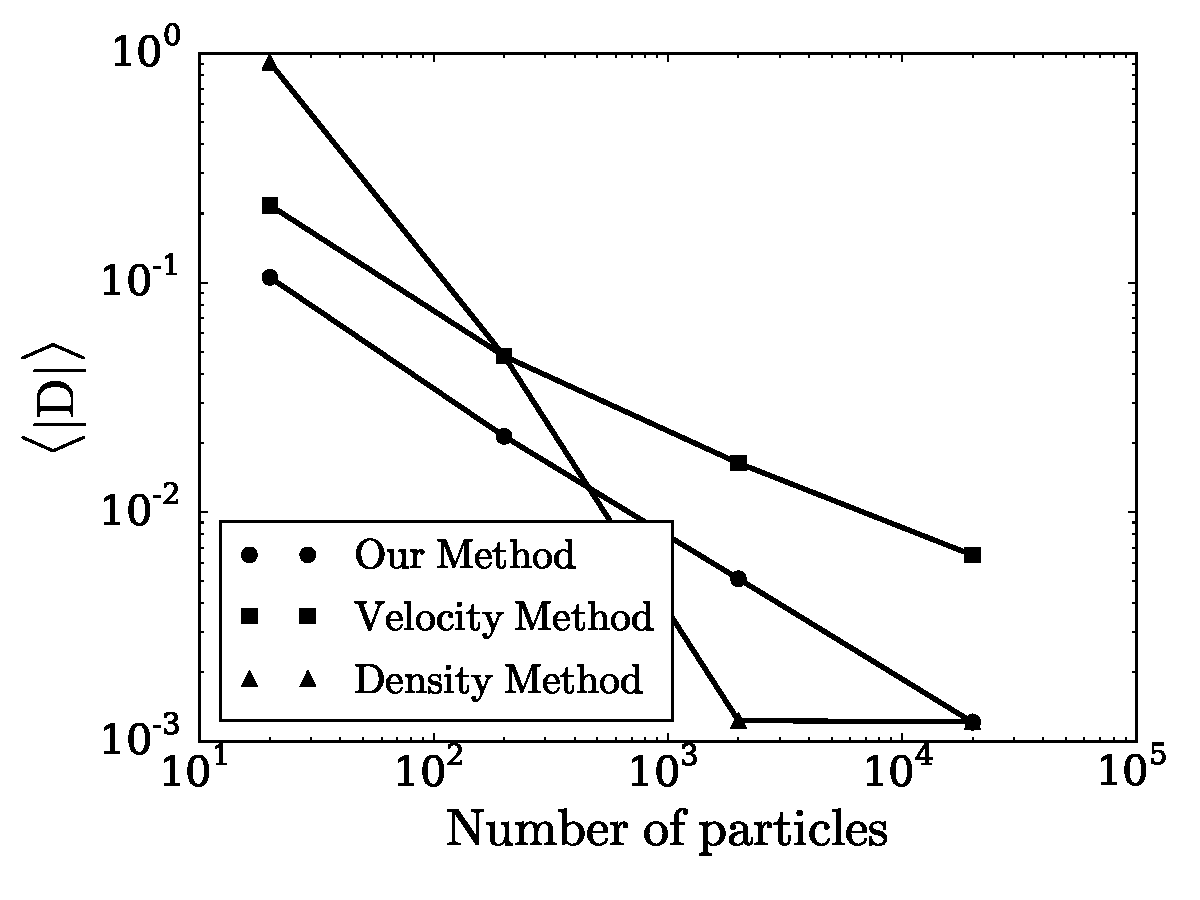
\includegraphics[width=0.70\textwidth]{error.pdf}
\end{center}
\caption{Average value of the relative error in the concentration
  estimate, $\avg{|D|}$, as a function of the particle number $N$ in
  the set of mock halos. Different symbols represent different
  methods. Our method provide the most accurate estimate at fixed
  particle number $N$.
    \label{fig:error}}
\end{figure*}

Figure \ref{fig:error} shows the behaviour of $\avg{|D|}$ as a function of
halo particle number for the three different methods to estimate the
concentration.

At fixed particle numbers our method always shows the lowest
$\avg{|D|}$ values compared to the other two methods.
Its accuracy is on the order of $10\%$ for $20$ particles in the halo,
going down to $0.01\%$ for halos with $20000$ particles.
The dependence of $\avg{|D|}$ with the particle number $N$ goes
approximately as $\avg{|D|}\propto N^{-1/2}$, hinting that
the accuracy of the method is related to a decrease of Poisson
noise.

The method based on the maximum of the circular velocity shows a similar
behaviour $\avg{|D|}\propto N^{-1/2}$. 
Its accuracy is $2-5$ times less
than in our method, on the order of $20\%$ for $20$ particle halos and
$0.5\%$ for $20000$ particle halos. 
The method based on the direct density
fit shows the lowest accuracy for a low particle number and an intermediate
accuracy between the other two methods for a high particle number.

\subsection{Halos from a cosmological simulation}


\label{sec:data}
\begin{figure*}
  \begin{center}
    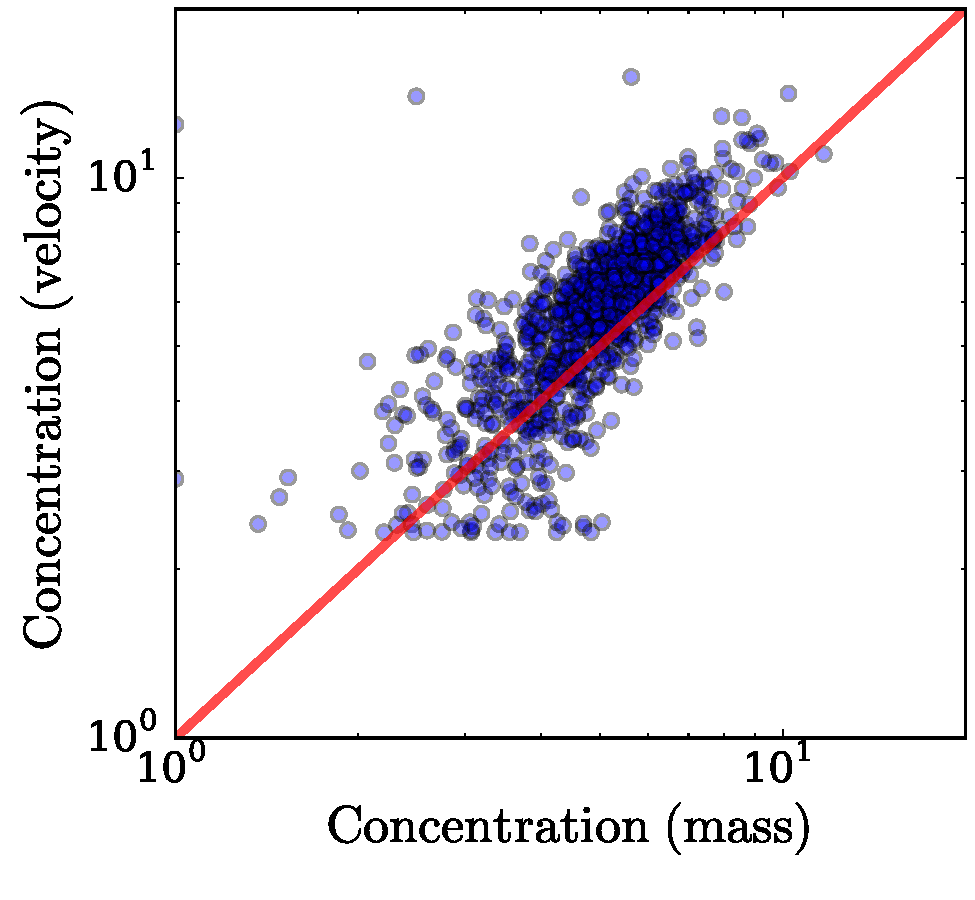
\includegraphics[width=0.33\textwidth]{conc_mass_vel.pdf}
    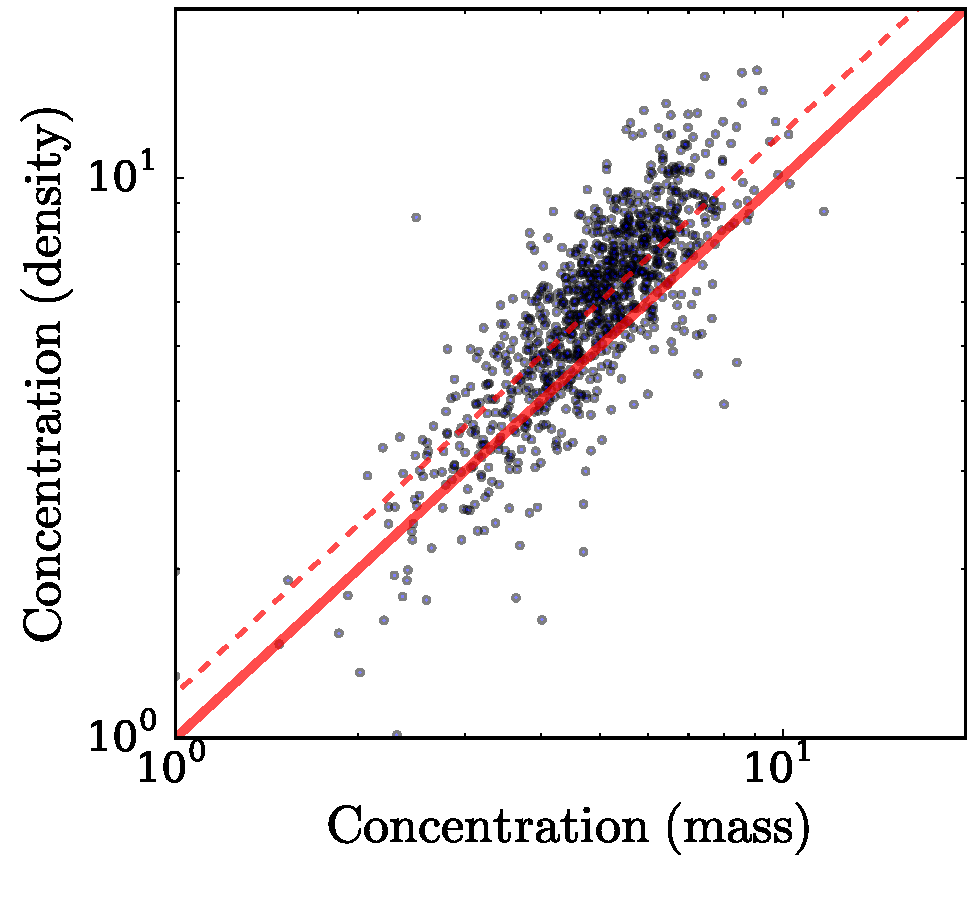
\includegraphics[width=0.33\textwidth]{conc_mass_dens.pdf}
    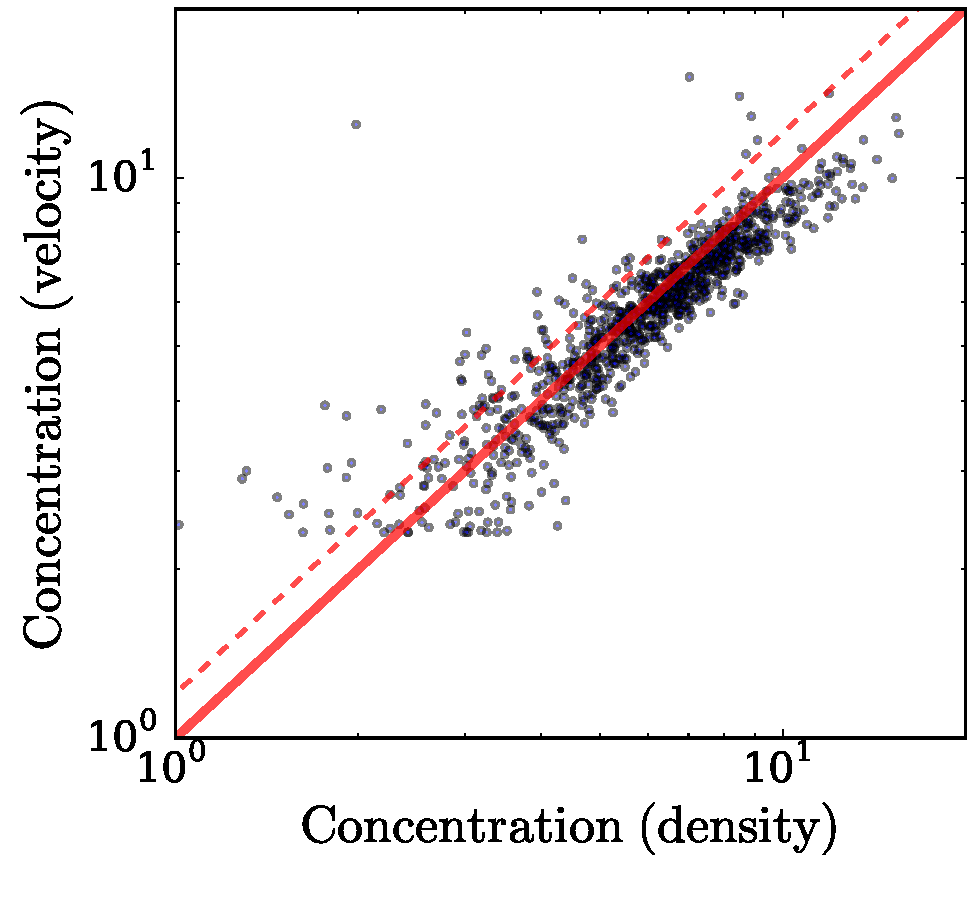
\includegraphics[width=0.33\textwidth]{conc_dens_vel.pdf}
  \end{center}
  \caption{Comparison between the concentrations measured by our
    method and the maximum velocity (left) and density (middle)
    methods. The line indicates the equal value between the two
    techniques. The right panel compares the results of the maximum
    velocity and density methods.
  \label{fig:mdv}}
\end{figure*}


We use data from the MultiDark cosmological simulation that follows
the non-linear evolution of a dark matter density field sampled with
$2048^3$ particles over a cubic box of $1000$ \hMpc on a side. 
The data is publicly available through \url{http://www.cosmosim.org/}.
More details about the structure of the database and the simulation
can be found in \citep{2013AN....334..691R}.

We build a sample of all halos located in a cubic sub-volume of $100$
\hMpc on a side centered on the most massive halo in the simulation at
$z=0$ which corresponds to the \texttt{miniMDR1} tables in the
database.
From this sample we select all the halos at $z=0$ detected with a
Friends-of-Friends (FoF) algorithm with masses in the interval
$10^{12}\leq M_{\rm FoF}/\hMsun \leq 10^{15}$.
The FoF algorithm used with a linking length of $0.17$ times the average
inter-particle distance. This choice translates into an overdensity
$\Delta_h\sim 400-700$ dependent on the halo concentration
\citep{More2011}.
Finally, we select from the database all the particles that belong to
each FoF group.

From this set of particles we follow the procedure spelled out in
Section \ref{sec:method} with $\Delta_h=740$  (corresponding to $200$
times the critical density) to select an spherical region that we
redefine to be our halo.
This choice makes that our overdensities are fully included inside the
original FoF particle group.
On the interest of providing a fair comparison against the density
method we only report results from overdensities with at least $200$
particles. 

Figure \ref{fig:concentration} shows the results of the
mass-concentration relationship.

\begin{figure*}
\begin{center}
  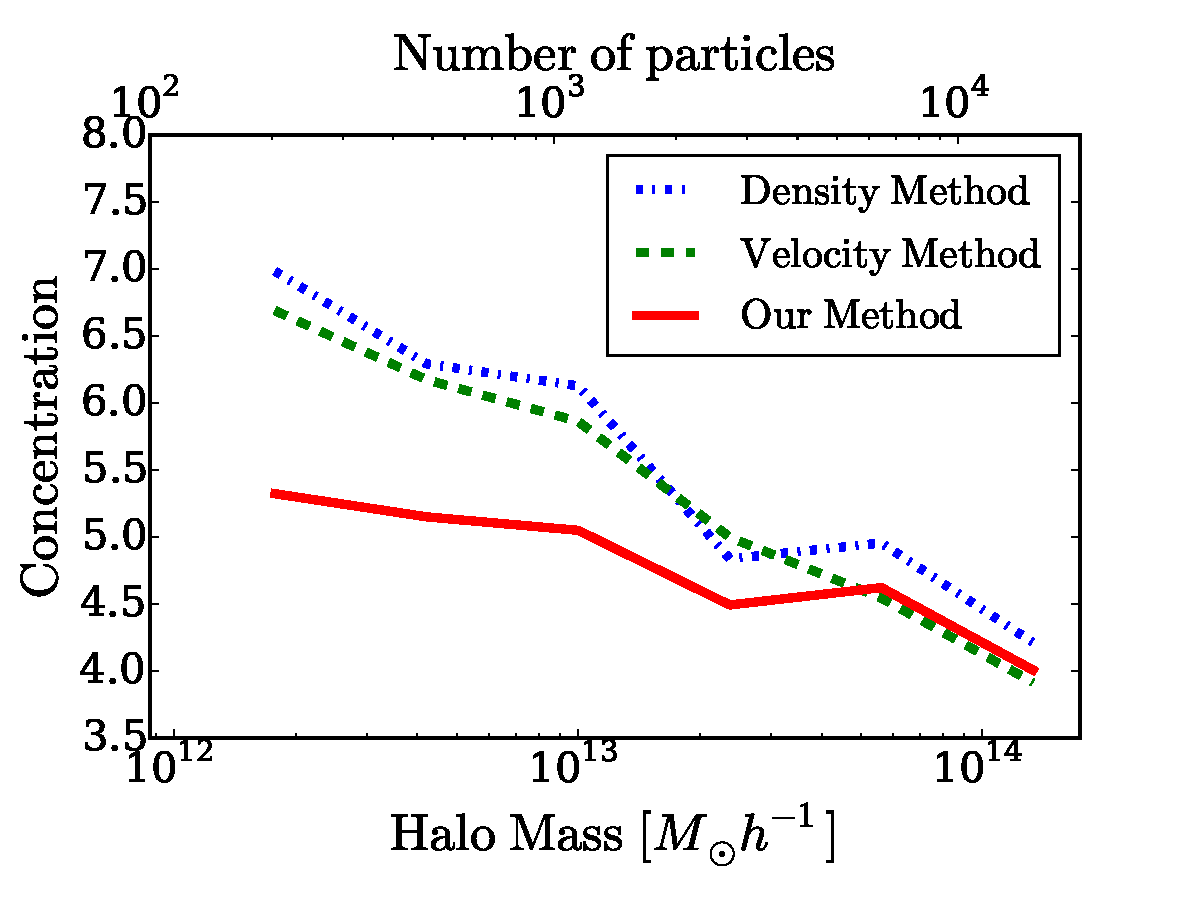
\includegraphics[width=0.75\textwidth]{concentration.pdf}
\end{center}
\caption{Mass-concentration relationship for the three different
  methods used on the same cosmological N-body data. 
  The lines correspond to the median concentration values in each bin.
    \label{fig:concentration}}
\end{figure*}



\section{Conclusions}
\label{sec:conclusions}

In this paper, we presented a new method to estimate the
concentration of dark matter halos in N-body simulations. 
We tested our method on mock halo data to study the impact of total
number of particles and input concentration on the retrieved values.
We compared these results against two other methods commonly used in
the literature to estimate concentrations.
Finally, we applied our method to halos extracted from a cosmological
N-body simulation to estimate the impact of our method on the mass
concentration relationship. 


The first benchmark was performed on mock halos generated with known
concentration values for different particle numbers. 
For all methods, the accuracy in retrieveing the input concentration
increases with the number of particles as summarized in Figure \ref{fig:error}.
Our method systematically shows smaller errors in the retrieved values
compared to the other two methods, going from $10\%$ for halos with
$20$ particles down to $0.01\%$ for halos with $2\times 10^4$ particles. 
In our method the average error on the retrieved values decreases with
the number of particles as $\langle|D|\rangle\propto N^{-1}$.
The error in density method initially behaves as $\langle|D|\rangle\propto
N^{-3/2}$ but at $N=2\times 10^3$ it saturates to $0.1\%$. 
For the velocity method the error behaves closely to
$\langle|D|\rangle\propto N^{-1/2}$.
We also gauged the effect of different concentration parameters at
fixed particle numbers. 
We found larger offsets for larger input concentrations. 
The offset goes in the sense that the measured concentration tends to
be underestimated.
Nevertheless, the dominant effect on the measurement is the particle
number.

We used a N-body cosmological simulation to test the impact of our
method on the mass-concentration relationship.
Although the three methods are in general agreement there are
noticeable differences in the mass concentration relationship.



\bibliographystyle{mn2e}
\bibliography{references}

\end{document}


